\documentclass[a4paper,12pt]{scrreprt}
    %% Used for changing geometry of the page
    %% Cover page text cannot overlay cover sketching/style
    %% https://ctan.org/pkg/geometry?lang=en
\usepackage{geometry}
    %% Changes language of some packages protocols
    %% e.g., when captioning images: Figure 1. -> Figura 1.
    %% https://ctan.org/pkg/babel?lang=en
\usepackage[portuguese]{babel}
    %% Used for special fonts
    %% Cannot be compiled with pdflatex
    %% https://ctan.org/pkg/fontspec?lang=en
\usepackage{fontspec}
    %% Arial FONT
    \setmainfont{Arial}

    %% More colors and color options
    %% https://ctan.org/pkg/xcolor?lang=en
    %% https://ctan.org/pkg/colortbl?lang=en
\usepackage{xcolor,colortbl}
    %% More tabular options, like dashed/dotted lines
    %% https://ctan.org/pkg/arydshln?lang=en
\usepackage{arydshln}
    %% List of acronyms
    %% https://ctan.org/pkg/nomencl?lang=en
\usepackage[intoc]{nomencl}
    %% Must be called to init nomencl environment
    \makenomenclature
    %% More images options/settings
    %% https://ctan.org/pkg/graphicx?lang=en
\usepackage{graphics}
    %% Defining subdirectories to image path enviornment
    %% \graphicspath{{sub1}{sub2}...{subN}}
    \graphicspath{{images}}

    %% used to handle cross-referencing commands in LaTeX to produce hypertext links in the document
    %% https://ctan.org/pkg/hyperref?lang=en
\usepackage{hyperref}
    %% math environments
    %% https://ctan.org/pkg/amsmath?lang=en

    %% settings
    \hypersetup{
        colorlinks,
        citecolor=black,
        filecolor=black,
        linkcolor=black,
        urlcolor=black
    }

\usepackage{amsmath}
    %% Defining backgrouns, used to make the cover
    %% https://ctan.org/pkg/background?lang=en
\usepackage[some]{background}
    %% Used to make drawings or complex graphics
    %% http://pgf.sourceforge.net/pgf_CVS.pdf
\usepackage{tikz}
    %% Tikz library to point operations ((x1,y1) + (x2,y2))
    \usetikzlibrary{calc}

%% Defining sfdefault font and default font for document
\renewcommand{\familydefault}{\sfdefault}

%==========================================================================
% DOCUMENT
%==========================================================================

\begin{document}

\pagenumbering{gobble}

%% Costume made cover
%% From there you can use \makecover command to build the cover
%% Blue cover color
\definecolor{titlepagecolor}{RGB}{208,112,68}

%==========================================================================
% COLORED BAR ON THE LEFT SIDE
%==========================================================================

\backgroundsetup{
    scale=1,
    angle=0,
    opacity=1,
    contents={
        \begin{tikzpicture}[remember picture,overlay]
            \path [fill=titlepagecolor] (-10.5,-15) rectangle ++ (5,30);
            \node[color=white] at (-7,-12) {\bfseries {\fontsize{120}{60} \textsf{P}}};
            \node[color=titlepagecolor] at (-4,-12) {\bfseries {\fontsize{120}{60} \textsf{O}}};
            \node[color=titlepagecolor] at (-1,-12) {\bfseries {\fontsize{120}{60} \textsf{O}}};
        \end{tikzpicture}
    }
}

%==========================================================================
% TITLE PAGE INFO
%==========================================================================

%% Changes values in this field to show information in the cover and back cover about your team/project

%% TITLE
\title{TODO - title}

%% AUTHORS
\author{
    Flávia Alexandra Silva Araújo (A96587) \\
  \quad
    Miguel Torres Carvalho (A95485)
}

%% Date

\date{\today}

%% Course
\newcommand{\Course}{Licenciatura em Engenharia Informática}

%% Department
\newcommand{\Department}{Escola de Engenharia}

%% UniName
\newcommand{\UniName}{Universidade do Minho}

%% UniPic
\newcommand{\UniPic}{
\includegraphics[scale=0.5]{images/eeum.png}}

%% University
\newcommand{\University}{
    \begin{flushleft}
        \UniPic
    \end{flushleft}
    \textcolor{gray}{\small\textbf{\textsf{\UniName}}}\par
    \textcolor{gray!80!white}{\small{\textsf{\Department}}}\par
    \textcolor{gray!70!white}{\small{\textsf{\Course}}}
}

%% UC
\newcommand{\UC}{
    \begin{flushleft}
        \par\textcolor{titlepagecolor}{  \LARGE\textbf{\textsf{Unidade Curricular de \\ Programação Orientada a Objetos}}}
    \end{flushleft}
}

%% School Year
\newcommand{\SchoolYear}{
    \small{\textsf{Ano Letivo de 2023/2024}}}


%% Define new command to show title, author and date
\makeatletter
\let\Title\@title
\let\Author\@author
\let\Date\@date
\makeatother

%==========================================================================
% CLASSIFICATION SECTION
%==========================================================================

%% School Year
\newcommand{\ReceptionDate}{}
%% Responsible
\newcommand{\Responsible}{}
%% Evaluation
\newcommand{\Evaluation}{}
%% Observations
\newcommand{\Observations}{}

%% MAKETEMPLATE
\newcommand{\makecover}{

%==========================================================================
% BEGIN COVER PAGE
%==========================================================================

%% Removes page number on footer
\thispagestyle{empty}

%% No indentation
\setlength{\parindent}{0em}

%% Put Background defined on \backgroundsetup, in this page
\BgThispage

%% Changing geometry to prevent overlay with text
%% At the end of back cover, geometry is default with \restoregeometry
\newgeometry{top=5cm,left=6cm,right=3cm,bottom=2cm}

%% builds university info defined previously
\University
\vspace{1cm}
%% builds curricular unity info defined previously
\UC
%% builds school year info defined previously
\SchoolYear

\vspace*{5cm}
%% bigger space (i think its the default one) between paragraphs
\setlength{\parskip}{1em}

%% builds title info defined previously
\par\textbf{\textsf{\huge\Title}}
\vspace{1cm}
%% builds author(s) info defined previously
\par\Author

\vspace{0.5cm}

%% builds date info defined previously
\par\Date
\restoregeometry
\pagebreak

%==========================================================================
% END COVER PAGE
%==========================================================================

%==========================================================================
% BEGIN BACK COVER PAGE
%==========================================================================

%% Removes page number on footer
\thispagestyle{empty}

\textbf{Equipa de Trabalho:}

% \begin{center}

\includegraphics[scale=0.5]{images/flavia.png} \\
\textbf{Flávia Alexandra Silva Araújo (A96587)} \\ \\

\includegraphics[scale=0.5]{images/miguel.png} \\
\textbf{Miguel Torres Carvalho (A95485)}
% \end{center}

\pagebreak
%==========================================================================
% END BACK COVER PAGE
%==========================================================================
}


% builds the cover
\makecover

%% smaller footer and header size
\newgeometry{top=3cm,left=3cm,right=3cm,bottom=4cm}
\savegeometry{default}

%==========================================================================
% BEGIN ABSTRACT PAGE
%==========================================================================

% Abstract name: \Large font size, flushed left and paragraph skip before abstract content
\renewenvironment{abstract}
 {\par\noindent\textbf{\Large\abstractname}\par\bigskip}
 {}

\begin{flushleft}
\begin{abstract}
    No âmbito da Unidade Curricular Programação Orientada a Objetos, foi-nos proposto o 
    desenvolvimento de uma aplicação de gestão de atividades físicas, à qual chamámos \textit{Activity Planner}. 
    A aplicação desenvolvida permite a gestão de utilizadores, atividades, planos de treino, simulação de atividades e 
    visualização de estatísticas. A aplicação foi desenvolvida em \textit{Java}, utilizando o paradigma de programação 
    orientada a objetos aprendido nas aulas. Neste relatório, é apresentada a arquitetura de classes da aplicação, bem 
    como as funcionalidades implementadas nesta e a forma como as mesmas foram desenvolvidas.
\end{abstract}
\end{flushleft}

%==========================================================================
% END ABSTRACT PAGE
%==========================================================================

%==========================================================================
% BEGIN INDEXES PAGES
%==========================================================================

%% Changes table of content name
%% Portuguese babel default : "Conteúdo"
%% Personally I prefer "índice"
\renewcommand{\contentsname}{Índice}
% \renewcommand{\listfigurename}{Índice de Figuras}
% \renewcommand{\listtablename}{Índice de Tabelas}

\tableofcontents

\pagebreak

% \listoffigures
%
% \pagebreak
%
% \listoftables
%
% \pagebreak

%==========================================================================
% END INDEXES PAGES
%==========================================================================

%==========================================================================
% BEGIN ARQUITETURA DE CLASSES
%==========================================================================

%% Starting page numbering here
\pagenumbering{arabic}

\chapter{Arquitetura de Classes}
\section{Diagrama de Classes}
\textcolor{red}{
    Descrever o diagrama de classes da aplicação, apresentando as classes e as suas relações.
}

\newgeometry{top=1.5cm,left=0.2cm,right=0.2cm,bottom=3.5cm}
\begin{center}
    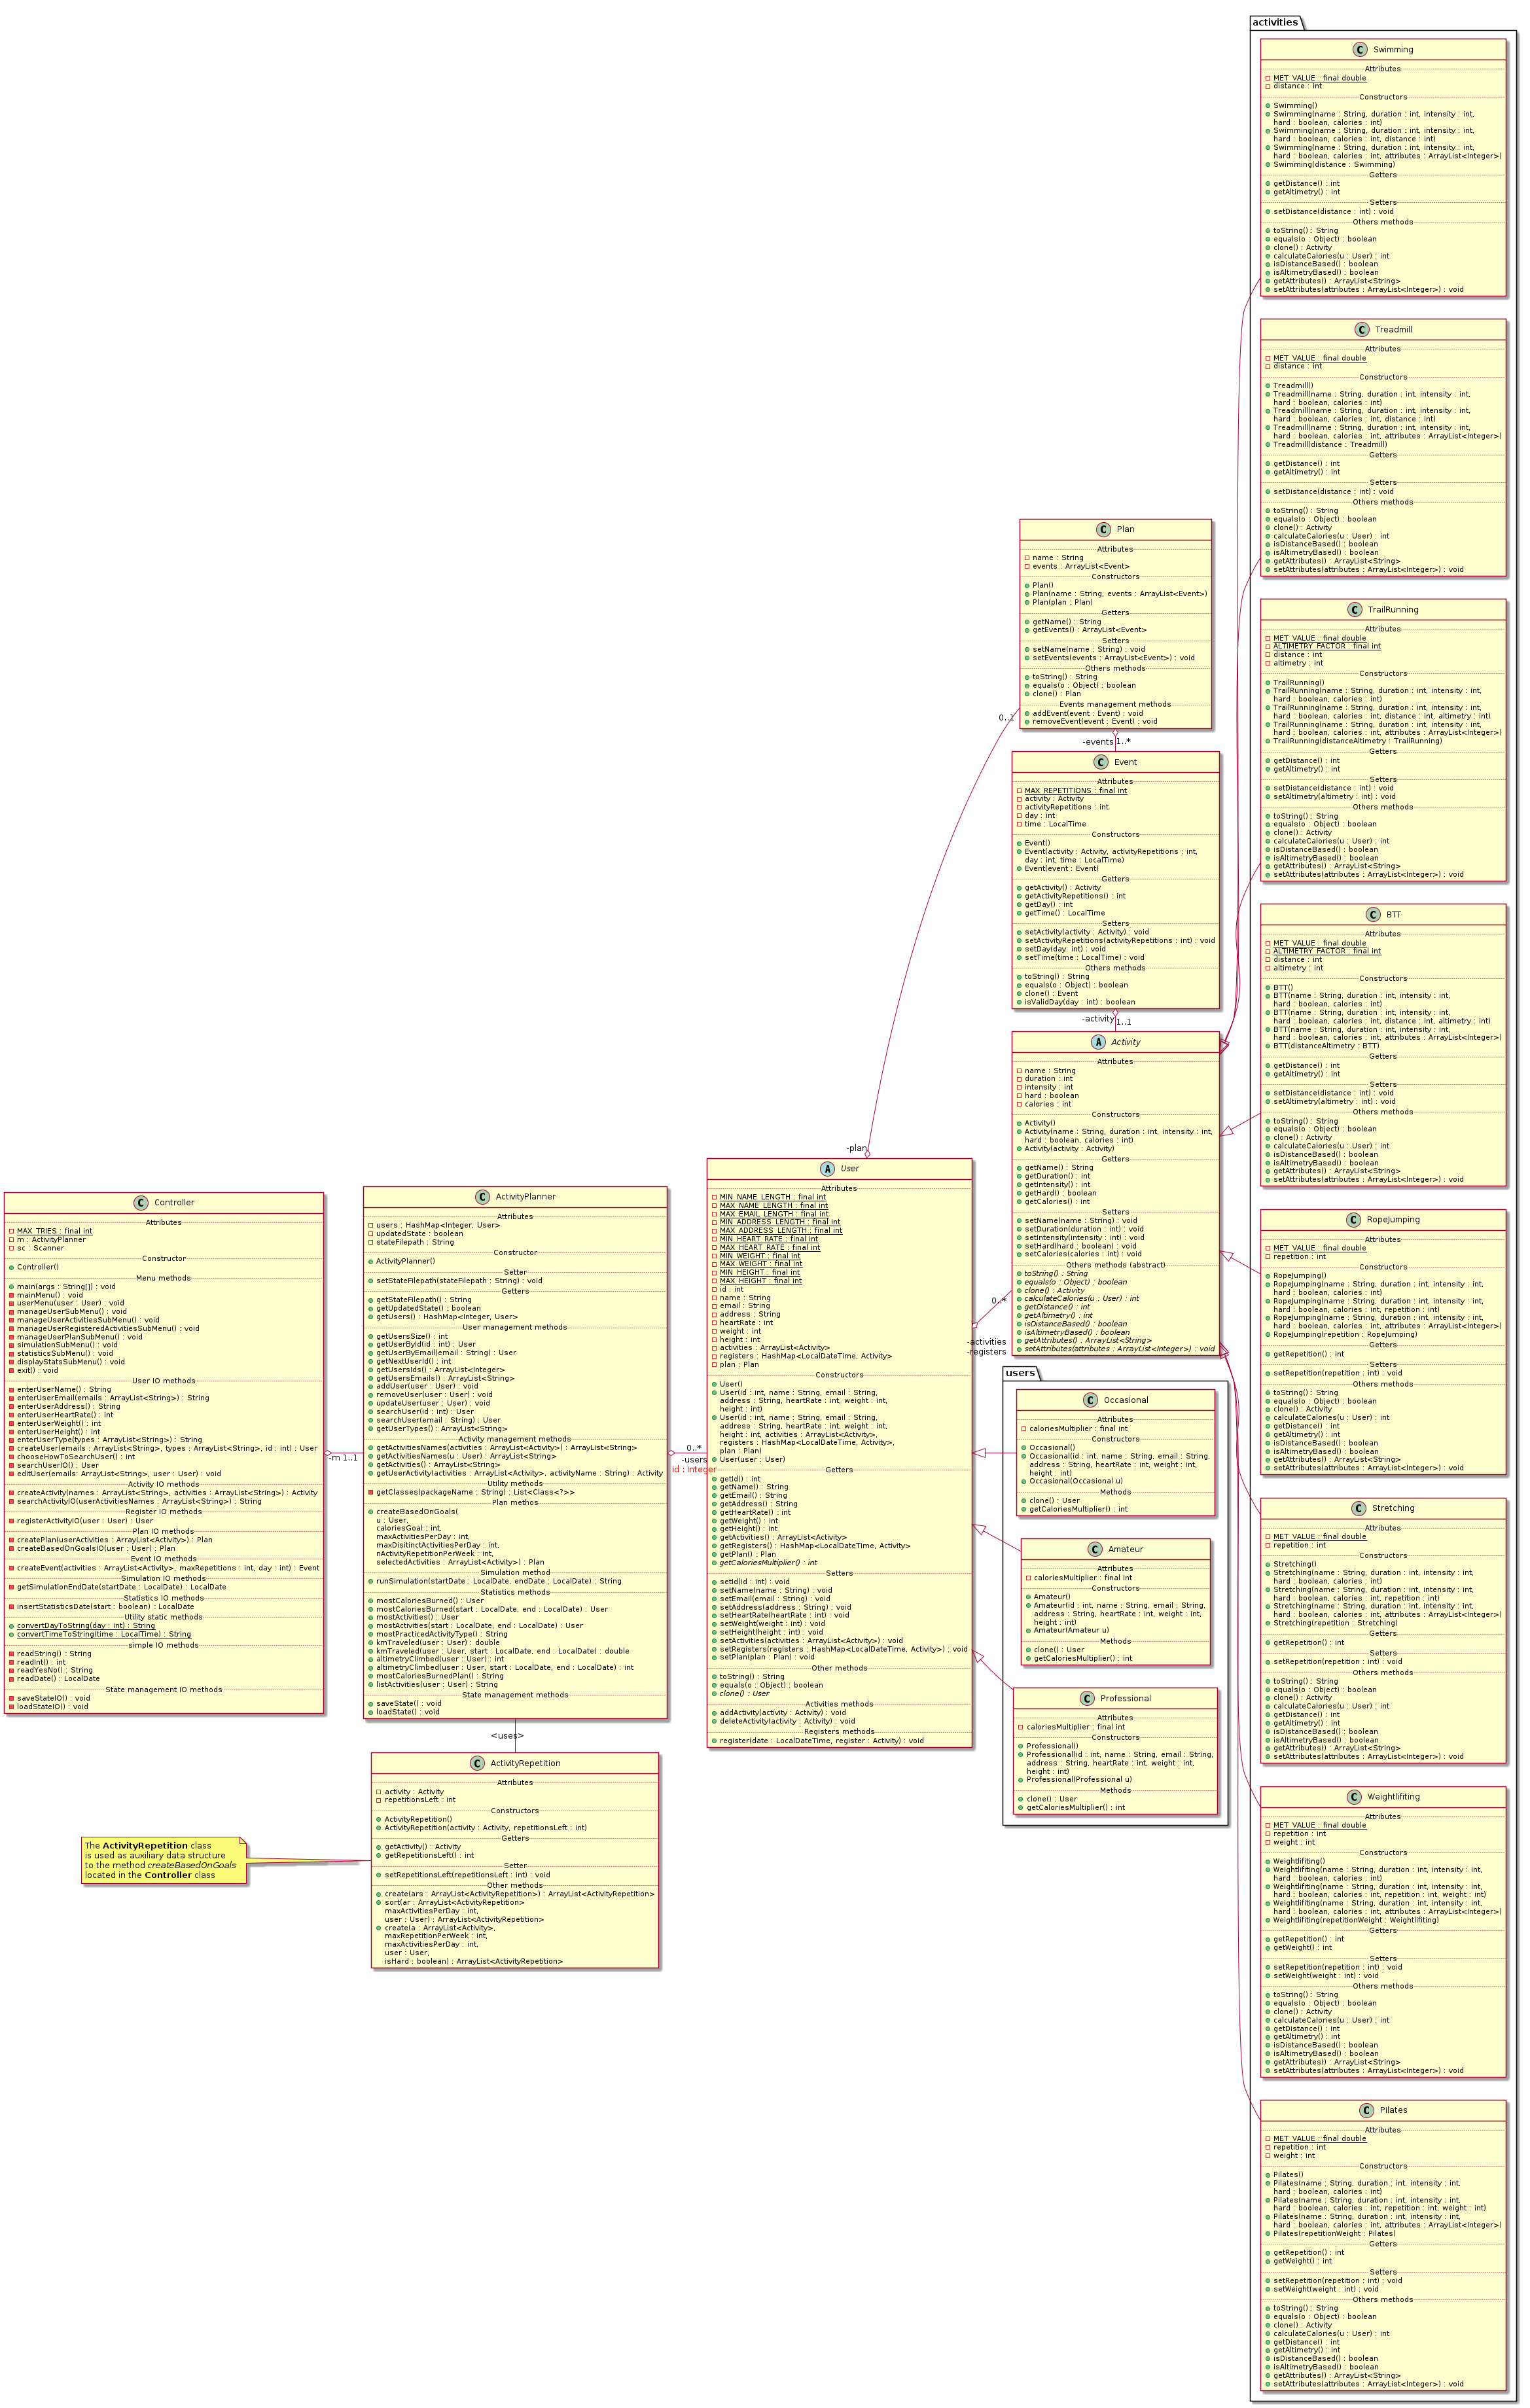
\includegraphics[scale=0.25]{images/diagram.png}
\end{center}
\loadgeometry{default}

\section{Classe \textit{Main}}
\section{Classe \textit{User}}
\section{Classe \textit{Activity}}
\section{Classe \textit{Event}}
    A classe \textit{Event} representa um evento correspondente a um plano de treino, sendo constituída pelos seguintes atributos:

    \begin{itemize}
        \item \textit{\textbf{activity : Activity}} - Atividade praticada no evento;
        \item \textit{\textbf{activityRepetitions : int}} - Número de vezes que a atividade será praticada;
        \item \textit{\textbf{day : int}} - Dia da semana do evento, onde 1 corresponde a domingo e 7 a sábado;
        \item \textit{\textbf{time : LocalTime}} - Hora do evento.
    \end{itemize}

\section{Classe \textit{Plan}}
    A classe \textit{Plan} representa um plano de treino, por definição, semanal, que um utilizador pode criar, vizualizar e remover.

    Esta é composta pelos seguintes atributos:
    \begin{itemize}
        \item \textit{\textbf{name : String}} - Nome do plano de treino;
        \item \textit{\textbf{events : ArrayList<Event>}} - Lista de eventos que compõem o plano de treino.
    \end{itemize}

    Para além dos vários construtores, dos métodos tradicionais de acesso e modificação dos atributos (\textit{getters} e \textit{setters}), métodos para a cópia profunda dos objetos desta classe, conversão para \textit{String} e
    igualdade entre objetos desta classe, foram implementados métodos para a adição de um evento a um plano de treino, para a criação interativa de um plano e para a criação de um plano baseado nos objetivos de um utlizador.

    As funcionalidades proporcionadas por esta classe serão detalhadas no capítulo \textit{\nameref{sec:gestao-planos-treino}}.

\section{Classe \textit{Stats}}

\section{Classe \textit{Simulation}}

\section{Classe \textit{IO}}
    No âmbito de agilizar a coleta de \textit{input's} por parte de um utilizador, foi criada a classe \textit{IO}, com os seguintes métodos:

    \begin{itemize}
        \item \textit{\textbf{readString(sc : Scanner) : String}} - Método que lê uma \textit{String} introduzida pelo utilizador;
        \item \textit{\textbf{readInt(sc : Scanner) : Int}} - Método que lê um inteiro introduzido pelo utilizador;
        \item \textit{\textbf{readYesNo(sc : Scanner) : String}} - Método que lê um caracter introduzido pelo utilizador, que deverá ser `y` ou `n`, independentemente deste ser maiúsculo ou minúsculo.
    \end{itemize}

    Nestes métodos, é feita a validação do \textit{input} através da verificação das exceções lançadas pela classe \textit{Scanner}.

%==========================================================================
% END ARQUITETURA DE CLASSES
%==========================================================================

%==========================================================================
% BEGIN DESCRIÇÃO DE FUNCIONALIDADES DA APLICAÇÃO
%==========================================================================

\chapter{Descrição de Funcionalidades da Aplicação}

\section{Gestão de Utilizadores}
    \subsection{Adicionar Utilizador}
    \subsection{Editar Utilizador}
    \subsection{Remover Utilizador}
    \subsection{Visualizar Utilizadores}

\section{Gestão de Atividades}
    \subsection{Adicionar Atividade}
    \subsection{Remover Atividade}
    \subsection{Visualizar Atividades}

\section{Registo e Visualização de Atividades Completas}
    \subsection{Registar Atividade}
    \subsection{Visualizar Registos de Atividades}

\section{Gestão de Planos de Treino}
    \label{sec:gestao-planos-treino}
    \subsection{Adicionar Plano de Treino Interativamente}
    \subsection{Adicionar Plano de Treino Baseado em Objetivos}
    \subsection{Remover Plano de Treino}
    \subsection{Visualizar Planos de Treino}

\section{Simulação}

\section{Estatísticas}

\clearpage
\section{Salvaguarda do Estado da Aplicação}
Para garantir que o estado da aplicação é preservado entre execuções, esta
permite guardar e carregar o estado atual através de um ficheiro binário.
As opcões de guardar e carregar o estado do programa estão disponíveis no menu principal da aplicação. Adicionalmente o ficheiro binário pode ser carregado diretamente no início da execução do programa através da passagem da localização deste na linha de comandos.
Este ficheiro, por definição, é guardado na diretoria \textit{data} e tem o nome \textit{state.ser}, havendo a opção de carregar diferentes estados através da funcionalidade da linha de comandos supramencionada.

Para a implementação desta funcionalidade foram definidos dois métodos na classe \textit{Main}:
\begin{itemize}
    \item \textit{saveState} - Método que guarda o estado atual da aplicação num ficheiro binário, passado como argumento. Este método deteta se alguma mudança foi feita no estado do programa antes de a guardar, de forma evitar salvar o mesmo estado.
    \item \textit{loadState} - Método que carrega o estado da aplicação a partir de um ficheiro binário, passado como argumento.
\end{itemize}

Como os objetos da classe \textit{User} contêm referências para todos os objetos relevantes de serem guardados/carregados - lista de Atividades, conjunto de registos de atividades, Plano de treino semanal com os respetivos Eventos - foi necessário garantir que estes e a própria classe referente ao Utilizador implementassem a interface \textit{Serializable}, de forma a que fossem possíveis de ser guardados, e futuramente carregados, num ficheiro binário.

A aplicação também dispõe de uma capacidade inteligente de detetar mudanças no seu estado, através do atributo booleano \textit{updatedState} na classe \textit{Main}, o que permitiu a implementação das seguintes funcionalidades:

\begin{itemize}
    \item Notificar o utilizador de que o estado atual não foi guardado, caso este tente sair da aplicação, dando a opção de o guardar, caso o utilizador o deseje fazer.
    \item Notificar o utilizador que, ao carregar um novo estado, o estado atual será perdido, se houver alterações, dando a opção de retornar atrás se este não quiser perder o estado atual.
\end{itemize}

O valor do atributo \textit{updatedState} é incializado a \textit{false} no ínicio da execução do programa e é alterado para \textit{false} sempre que o estado da aplicação é guardado, no método \textit{saveState}, ou carregado, no método \textit{loadState}, referidos anteriormente.

Este valor booleano é alterado para \textit{true} sempre que o estado da aplicação é alterado, seja através da adição, edição ou remoção de um utilizador, de uma atualização de uma atividade de um utilizador, do registo de uma nova atividade ou da criação/remoção de um plano de treino para um utlizador em específico.

\section{Argumentos de Linha de Comandos}

%==========================================================================
% END DESCRIÇÃO DE FUNCIONALIDADES DA APLICAÇÃO
%==========================================================================

%==========================================================================
% BEGIN CONCLUSÕES DE TRABALHO FUTURO
%==========================================================================

\chapter{Conclusões e Trabalho Futuro}
    \textcolor{red}{
        Maybe
    }

%==========================================================================
% END CONCLUSÕES DE TRABALHO FUTURO
%==========================================================================

%==========================================================================
% BEGIN BIBLIOGRAFIA
%==========================================================================

%% Changes biblibography name
%% Portuguese babel default : "Bibliografia"
%% Personally I prefer "Referências"
% \renewcommand\bibname{Referências}

%% https://www.overleaf.com/learn/latex/bibliography_management_with_bibtex
% \begin{thebibliography}{9}
% \textcolor{red}{
%     <<Enumeração dos diversos recursos bibliográficos utilizados. Utilizar o sistema de referenciação APA (https://guias.sdum.uminho.pt/apa).>>
% }
% \end{thebibliography}

%==========================================================================
% END BIBLIOGRAFIA
%==========================================================================

%==========================================================================
% BEGIN LISTA DE SIGLAS E ACRÓNIMOS
%==========================================================================

%% Portuguese babel does not translate this environment
\renewcommand{\nomname}{Lista de Siglas e Acrónimos}

%% Text that can be shown before acronyms list
\renewcommand{\nompreamble}{
    \textcolor{red}{
        <<Apresentar uma lista com todas as siglas e acrónimos utilizados durante a realização do trabalho. O formato base para esta lista deverá ser da forma como abaixo se apresenta.>>
    }
}

%% acronyms
\nomenclature[01]{\textbf{POO}}{Programação Orientada a Objetos}

%% Show acronyms
\printnomenclature

%==========================================================================
% END LISTA DE SIGLAS E ACRÓNIMOS
%==========================================================================

%==========================================================================
% BEGIN ANEXOS
%==========================================================================

%% Why \addchap, instead of \chapter?
%% \addchap has no numbering but appears in table of contents.
% \addchap{Anexos}
%
%     \textcolor{red}{
%         <<Os anexos deverão ser utilizados para a inclusão de informação adicional necessária para uma melhor compreensão do relatório o para complementar tópicos, secções ou assuntos abordados. Os anexos criados deverão ser numerados e possuir uma designação. Estes dados permitirão complementar o Índice geral do relatório relativamente à enumeração e apresentação dos diversos anexos.>>
%     }
%
%     %% section version of \addchap
%     \addsec{Anexo 1}


%==========================================================================
% END ANEXOS
%==========================================================================
\end{document}
